%=============================================================================
% Datasets Appendix
% Copyright (c) 2018. Lester James V. Miranda
%
% This file is part of thesis-manuscript.
%
% thesis-manuscript is free software: you can redistribute it and/or modify
% it under the terms of the GNU General Public License as published by
% the Free Software Foundation, either version 3 of the License, or
% (at your option) any later version.
%
% thesis-manuscript is distributed in the hope that it will be useful,
% but WITHOUT ANY WARRANTY; without even the implied warranty of
% MERCHANTABILITY or FITNESS FOR A PARTICULAR PURPOSE.  See the
% GNU General Public License for more details.
%
% You should have received a copy of the GNU General Public License
% along with thesis-manuscript.  If not, see <http://www.gnu.org/licenses/>.
%
% Created by: Lester James V. Miranda <ljvmiranda@gmail.com>
%=============================================================================

\chapter{Dataset Description}
\label{AppendixDataset}

\par The two protein benchmarks, Yeast and Genbase, we used in this research
were from the works of \cite{elisseeff2001kernel} and
\cite{diplaris2005protein}.  Yeast contains micro-array expression data and
phylogenetic profiles with functions expressed as MIPS\footnote{ Munich
Information Center for Protein Sequences (\cite{mewes2006mips}) } annotations,
whereas Genbase consists of domain characterizations of various proteins and
their PROSITE IDs. Table \ref{setup:datasets} details these benchmarks.

\begin{table}[!h]
    \centering
    \caption{Dataset description}
    \label{setup:datasets}
    \begin{tabular}{@{}r*{8}{l}@{}}
        \toprule
        Dataset & Instances & Features & Labels & Card.    & Dens.   & MaxIR     & MeanIR   & CVIR     \\ \midrule
        yeast   & $2417$    & $103$    & $14$   & $4.237$  & $0.303$ & $53.412$  & $7.197$  & $1.884$  \\
        genbase & $662$     & $1186$   & $27$   & $1.252$  & $0.046$ & $171.000$ & $37.315$ & $1.449$  \\ \bottomrule
    \end{tabular}
\end{table}

\par We can use various metrics to describe a multilabel dataset
(\cite{charte2015imbalance}). As a preliminary, an active label is a binary
$1$, while a non-active label is binary $0$. A sample $n$ with a labelset
$\mathbf{y}_n = \left[1,0,1,0\right] (q=4, Y_n = \{\lambda_1, \lambda_3\})$ has
two active labels ($|Y_n|$). Thus, we have the following:
\begin{itemize}
    \item \textit{Cardinality}: the average number of active labels found per
        sample.
    \item \textit{Density}: the number of active labels with respect to all
        labels in the label-matrix.
    \item \textit{*IR}: statistical measurements of imbalance: max, mean, and
        variance.
\end{itemize}

\par Below are the equations for each metric:
\begin{align}
    \text{Card}(\mathcal{D}) &= \sum_{i=1}^{N}
    \dfrac{|{Y}_{i}|}{N} \\
    \text{Dens}(\mathcal{D}) &=
    \dfrac{\text{Card}(\mathcal{D})}{q} 
\end{align}

\par Data imbalance is one of the most common problems in machine learning,
especially when deploying models in the wild (\cite{he2009learning}). Whenever
one label dominates the other, the classifier becomes severely affected causing
it to only predict the majority label. This is felt in multilabel datasets,
although it not as pronounced in Yeast and Genbase (\cite{
charte2015imbalance}).  In our work, we used a label weighing scheme in the
classifier to offset this problem (\cite{pedregosa2011scikit,
chang2011libsvm}). To measure imbalance for a given label $\lambda$, we have
(\cite{charte2015imbalance}):
\begin{align}
    \text{IRLbl}(\lambda) =
    \dfrac{
        \text{argmax}_{\lambda^{\prime}=Y_1}^{Y_q}
        (\sum_{i=1}^{N} h(\lambda^{\prime},Y_i))
    }{
        \sum_{i=1}^{N} h(\lambda,Y_i)
    }, \quad h(\lambda, Y_i) =
    \begin{cases}
        1 & \lambda \in Y_i \\
        0 & \lambda \notin Y_i
    \end{cases} 
\end{align}

\par The equation looks like a handful, but the intuition is to find the ratio
between the majority and minority labels. The value is $1.00$ for
$\lambda_{\text{major}}$ and higher for the rest. If we have $20$ labels
($q=20$), then we have twenty measurements for IRLbl. We can then obtain their
mean, max, and variance to fill the MaxIR, MeanIR, and CVIR respectively.

\par Lastly, we can draw a co-occurence plot to visualize how difficult these
multilabel problems are. In Figure \ref{appendix:cooccurence}, each arc
represents a label while each chord represents the frequency that two labels
occured simultaneously in a given sample.

\begin{figure}[!h]
  \centering
  \begin{subfigure}[b]{0.48\textwidth}
    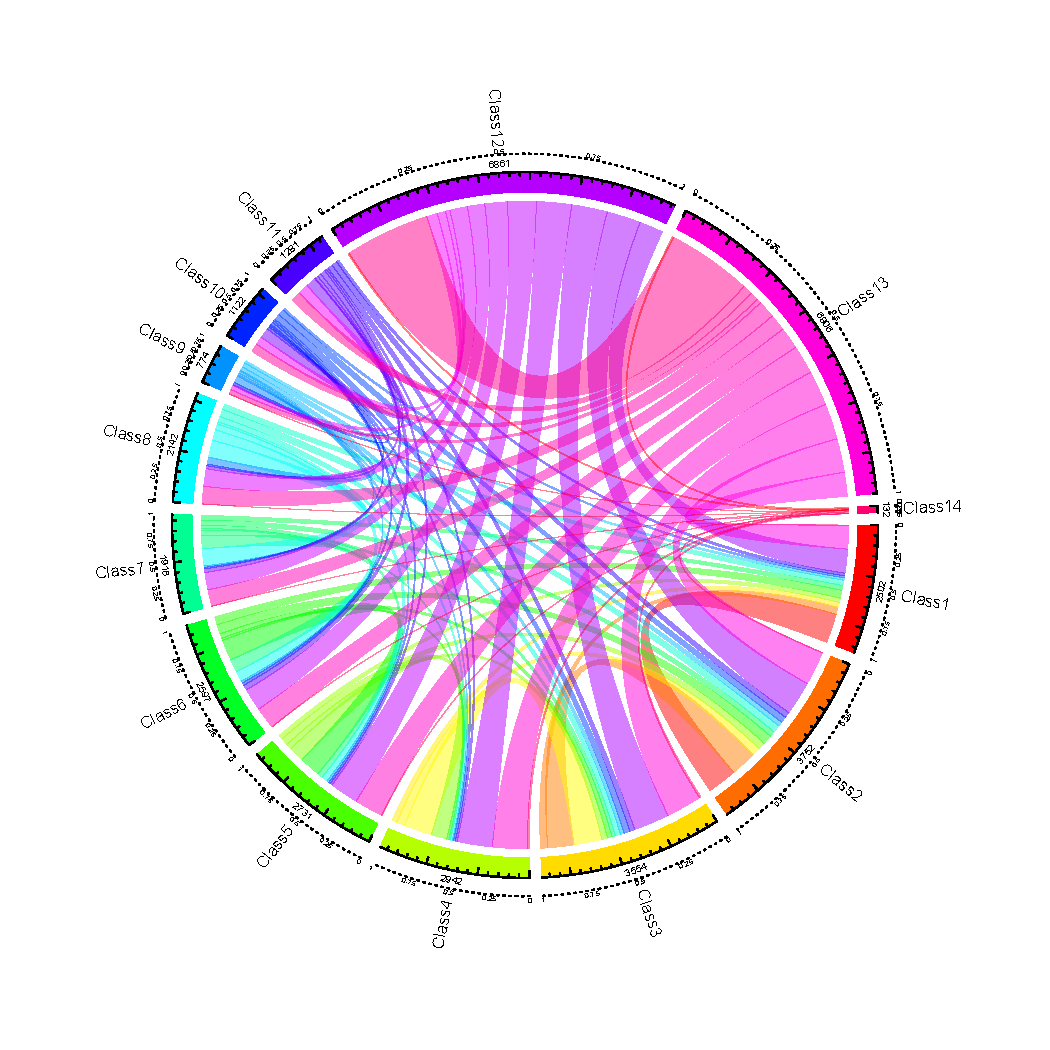
\includegraphics[width=\textwidth]{appendix/yeast_labelset}
    \caption{Yeast}
    \label{cooccurence:yeast}
  \end{subfigure}
  \begin{subfigure}[b]{0.48\textwidth}
    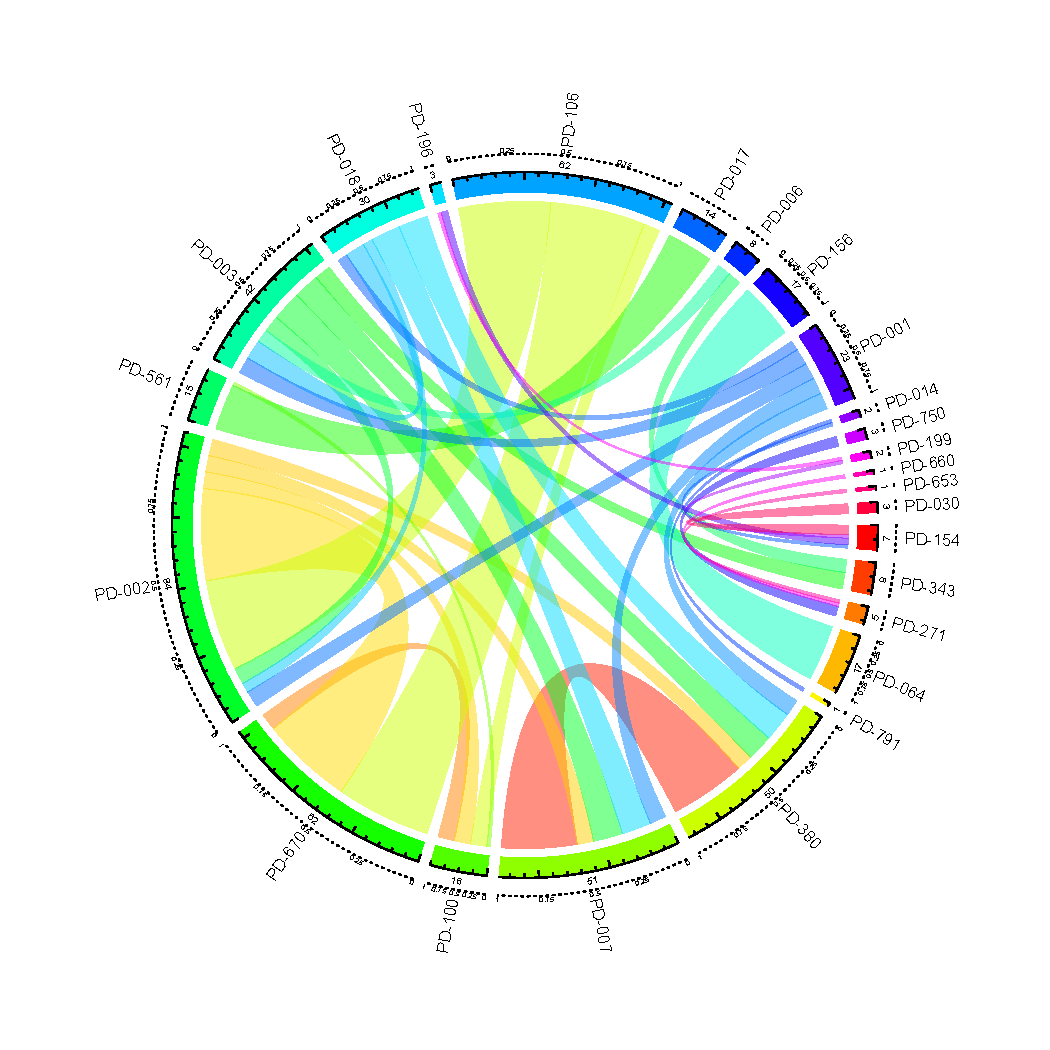
\includegraphics[width=\textwidth]{appendix/genbase_labelset}
    \caption{Genbase}
    \label{cooccurence:genbase}
  \end{subfigure}
  \caption{Cooccurence plot for protein benchmarks}
  \label{appendix:cooccurence}
\end{figure}

\par The work on multilabel data in general, not just in protein function
prediction, is a good area for further research (as addressed in Chapter
\ref{ConclusionsChapter}). It deals with problems not only in classification
but also  data imbalance and the like. For more information, we direct the
reader to the works of \cite{charte2015imbalance, charte2015mlsmote} and \cite{
charte2017dealing}
